\begin{refsection}[research/tomita/group.bib]
\nocite{*}
\chapter{Computational Climate Science Research Team}


\section{Members}

\begin{itemize}
  \item[] Hirofumi Tomita (Team Leader)
  \item[] Yoshiyuki Kajikawa (Senior Scientist)
  \item[] Shin-ichi Iga (Research Scientist)
  \item[] Seiya Nishizawa (Research Scientist)
  \item[] Hisashi Yashiro (Research Scientist)
  \item[] Sachiho Adachi (Research Scientist)
  \item[] Yoshiaki Miyamoto (Special Postdoctoral Researcher)
  \item[] Yousuke Sato (Postdoctoral Researcher)
  \item[] Tsuyoshi Yamaura (Postdoctoral Researcher)
  \item[] Ryuji Yoshida (Postdoctoral Researcher)
  \item[] Hiroaki Miura (Visiting Researcher)
  \item[] Mizuo Kajino (Visiting Researcher)
  \item[] Hiroshi Taniguchi (Visiting Researcher)
  \item[] Tomoko Ohtani (Research Assistant)
  \item[] Keiko Muraki (Research Assistant)
\end{itemize}

\section{Research Activities}

Our research team conducts the pioneering research work to lead the future climate simulation. In order to enhance the reliability of climate model more, we have aimed to construct a new climate model based on the further theoretically physical principles. Conducting such a new model needs tremendously large computer resources. Therefore, it is necessary to design the model to pull out the capability of computers as much as possible. Recent development of supercomputers has a remarkable progress. Hence another numerical technique should be needed under the collaboration of hardware research and software engineering for the effective use on the future HPC, including the K computer and Post K computer.

For the above research purpose and background, our team is cooperating with the computational scientists in other fields and computer scientists. We enhance the research and development for the future climate simulations including effective techniques; we build a next-generation climate model. The establishment of the above basic and infrastructure research on the K Computer is strongly required, because this research leads to the post K computer or subsequent ones in the future. 

We highlight the following studies in this fiscal year.
\begin{enumerate}
\item Construction of a new library for climate study:\\
We have proposed the subject “Estimation of different results by many numerical techniques and their combination” as a synergetic research to MEXT in 2011 through the discussion with the Strategic 5 fields (SPIRE). We develop a new library for numerical simulation. The progress in development of SCALE is reported. NICAM-DC was imported to SCALE as a global dynamical core in this fiscal year. The two landmark papers of the SCALE are reported.
\item Grand challenge run for sub-km horizontal resolution run by global cloud-resolving model:\\
Another outstanding simulation of global model NICAM on the K computer, with super-high resolution (870m), has been done. We analyze the simulation in cooperation with the SPIRE3. We report the further comprehensive analysis of convection properties in the simulation.
\item Disaster prevention research in establishment of COE project:\\
Hyogo-Kobe COE establishment project has accepted 5 subjects in 2012. One of subjects is ``the computational research of disaster prevention in the Kansai area''. In this subject, one of sub-subjects is “Examination of heavy-rainfall event and construction of hazard map”, which our team is responsible for. The tuning of physical properties focusing on the climatological precipitations and the preliminary result by direct downscaling are reported.
\end{enumerate}


\section{Research Results and Achievements}


\subsection{Construction of a new library for climate study}

We are working on research and development of a library (named SCALE) for numerical models in fluid dynamical field especially in meteorological field. We examined feasibility of numerical scheme and methods for developing new ones which are suite on massive parallel computers especially the K computer. In order to validate the schemes and test their performance in atmospheric simulations, we have been developing an atmospheric regional model (named SCALE-RM) as a part of the SCALE library. The SCALE library and the SCALE-RM are currently available as open source software at our web site (http://scale.aics.riken.jp/). It is also installed on the K computer and is available for the K computer users as an AICS Software (http://www.aics.riken.jp/en/kcomputer/aics-software.html). In this year, we continued to develop components which are necessary for real atmospheric simulations; a boundary turbulence scheme, an urban canopy model, nesting system, and preprocessing tools. We also have improved the library and the model for better performance in both physical and computational aspects. As a remarkable feature, NICAM-DC ( Nonhydrostatic ICosahedral Atmosphere Model Dynamical Core) was equipped to SCALE library as a global dynamical core. 

\begin{figure}
\centering
  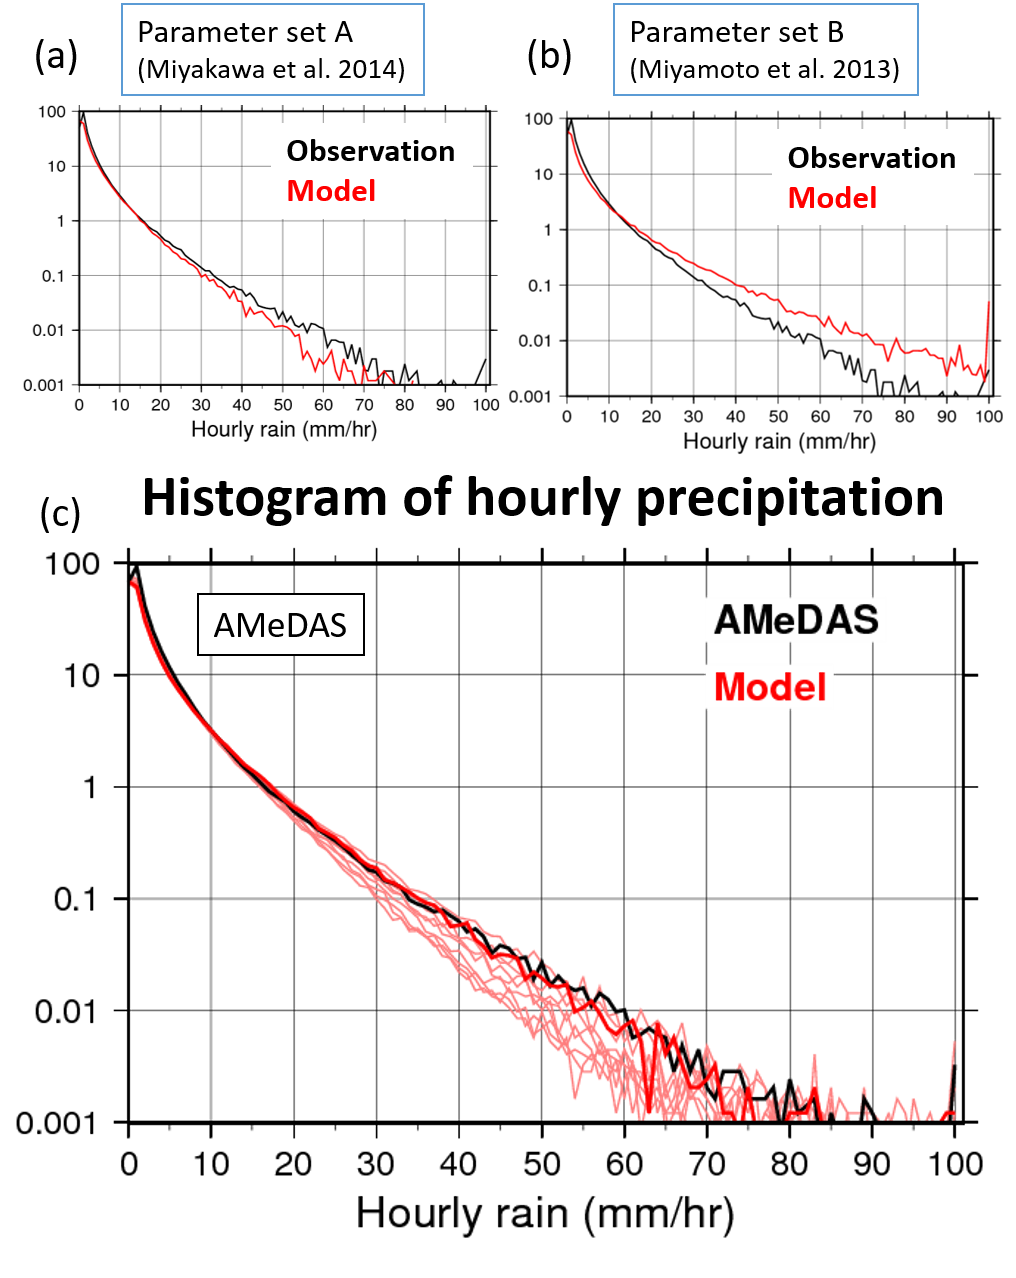
\includegraphics[width=0.5\textwidth,keepaspectratio,natwidth=193,natheight=40]
  {research/tomita/climate-teamFig1.png}
  \caption{Results of microphysics tuning.}
  \locallabel{fig:ctfig1}
\end{figure}


The validation for the physical performance is an important issue as well as code development. In this fiscal year, we tuned the microphysical scheme, focusing on the one-moment bulk method (Tomita et al.2008). Although this scheme was used also in NICAM through the project SPIRE, it depends on the resolution and phenomena we can see. For this purpose, we conducted the series of systematic parameter tuning suitable to Japanese western region using the GSM data as the boundary condition and compared the precipitation with AMeDAS data. Figure \localref{fig:ctfig1} (a) and (b) shows results of hourly precipitation histogram from two typical parameter sets of the microphysics, which has been used in NICAM experiments (Miyakawa et al. 2014, Miyamoto et al.2013). After several key parameters were swept, we successfully tuned the parameters as shown in Fig.\localref{fig:ctfig1} (c).




In this fiscal year, two landmark paper for SCALE was published. The first paper describes the proof-of-concept like study according to SCALE policy (Sato et al. 2015\cite{Sato_et_al_2015}). The three microphysical schemes, the one-moment bulk, two-moment bulk, and spectral bin schemes were compared by sensitivity experiments in which the other components were fixed in SCALE-RM. Since SCALE is targeting to enable self-model inter-comparison easily, this paper is high significant as a SCALE reference paper. The other paper is about the model description of SCALE-RM dynamical core(Nishizawa et al. 2015\cite{Nishizawa_et_al_2015}). In this paper, we reveals that the influence of the grid aspect ratio of horizontal to vertical grid spacing on turbulence in the planetary boundary layer (PBL) in a large-eddy simulation (LES). This paper gives a deep suggestion to meteorological LES. One key point is how the filter length be configured.  It should be based on consideration of the numerical scheme. We also confirmed necessity of a corrective factor for the grid aspect ratio into the mixing length. As shown in Fig.\localref{fig:ctfig2}, these remedy generates the theoretical slope of the energy spectrum; otherwise, spurious energy piling appears at high wave numbers.

\begin{figure}
\centering
  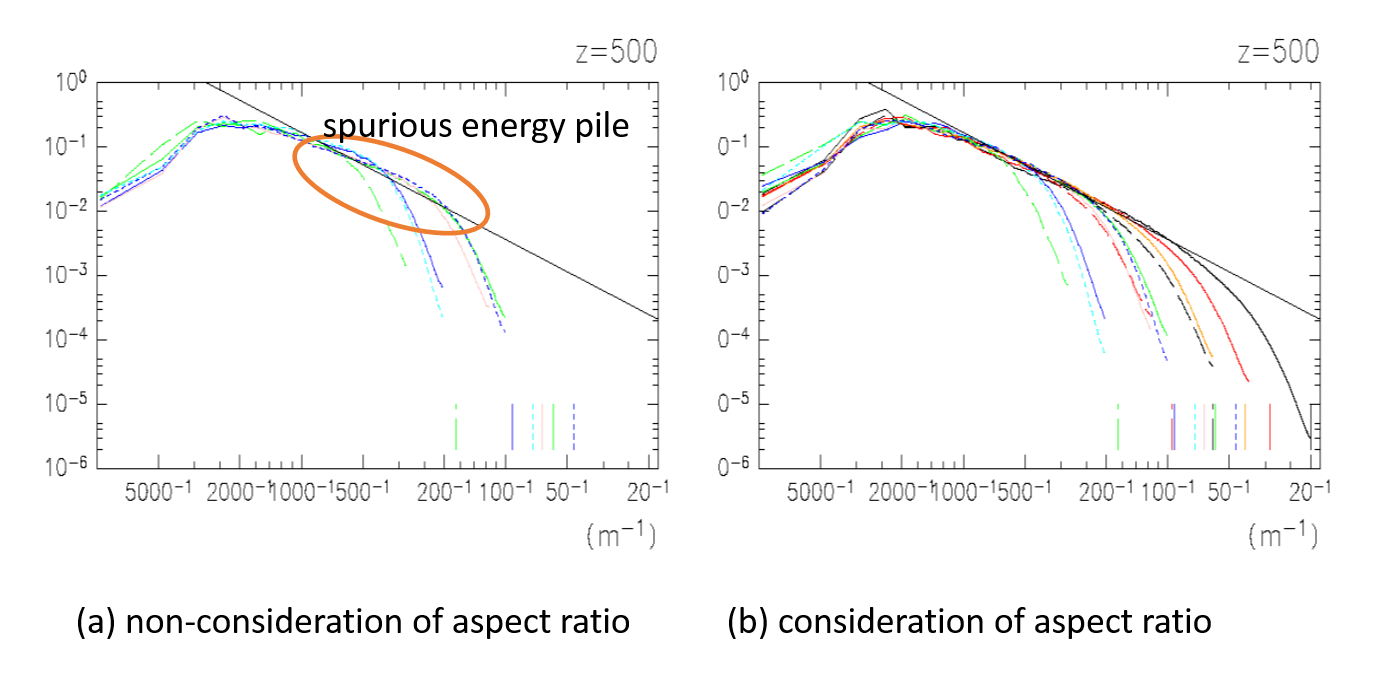
\includegraphics[width=0.8\textwidth,keepaspectratio,natwidth=193,natheight=40]
  {research/tomita/climate-teamFig2.png}
  \caption{The kinetic energy spectrum.}
  \locallabel{fig:ctfig2}
\end{figure}


We investigated also the computational performance of SCALE-RM from the viewpoint of strong scale.  Figure \localref{fig:ctfig4} shows the results of the strong scaling experiments for SCALE-LES. The most time-consuming part is the dynamics, and its scaling factor tends to be saturated by decreasing the problem size. This degradation comes from the increasing ratio of the communication time against the computational time. On the other hand, the scaling of physics gives relatively ideal scaling. In addition, the I/O part is not a bottleneck. To obtain the faster calculation, we implemented several choices both for the temporal and spatial difference schemes. As a result, the longer time step can be obtained in a certain configuration that is 4th order Runge-Kutta scheme in time and 3rd order advection scheme in space.

\begin{figure}
\centering
  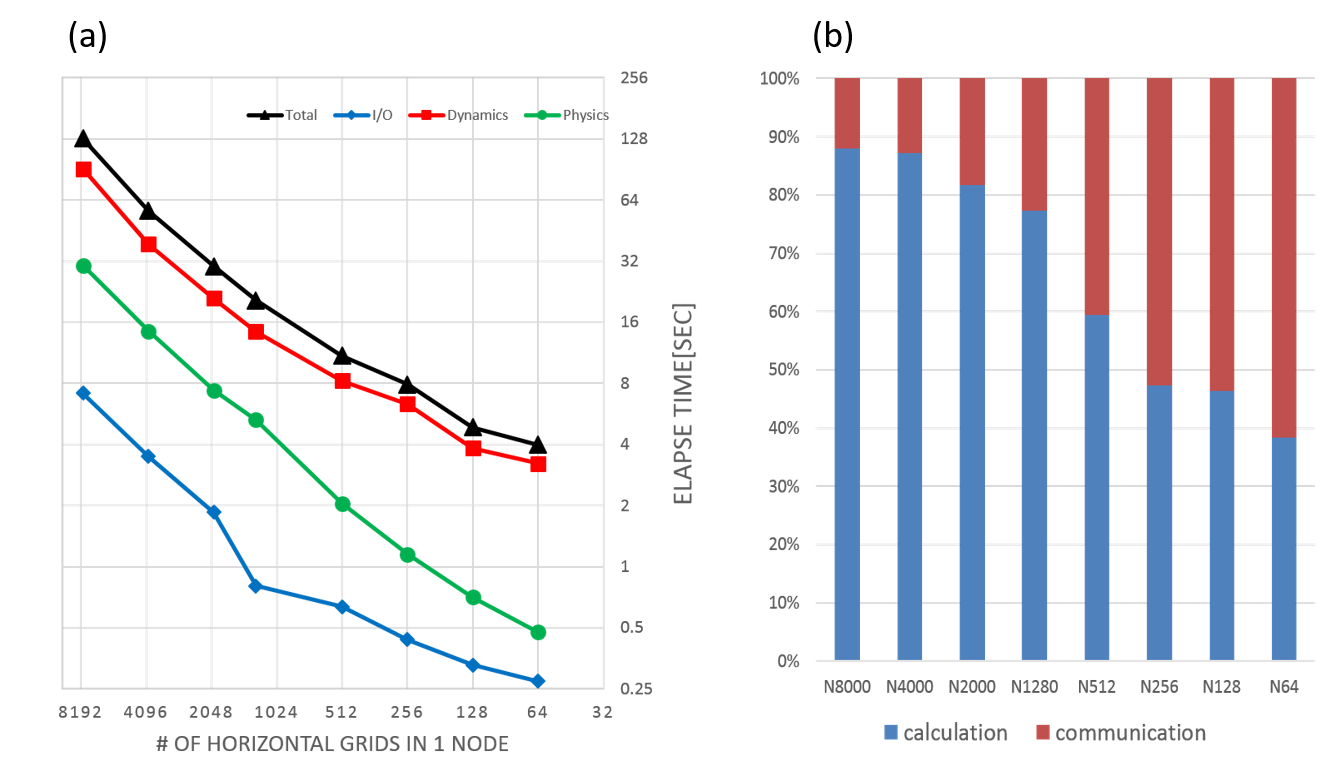
\includegraphics[width=0.8\textwidth,keepaspectratio,natwidth=193,natheight=40]
  {research/tomita/climate-teamFig4.png}
  \caption{(a) Strong scale of SCALE-RM. (b) Ratio of communication to calculation.}
  \locallabel{fig:ctfig4}
\end{figure}


\subsection{Grand challenge run for sub-km horizontal resolution run by global cloud-resolving model}
Using the K computer, we have succeeded in conducting the global simulation with the world’s highest resolution, 870 m, which is published in the 2013 fiscal year (Miyamoto et al. 2013).  In the fiscal year 2015, an additional analyses to reveal the differences in convection properties in various atmospheric disturbances has been done. We focused on the differences in convection under four representative cloudy disturbances: Madden-Julian Oscillation, Tropical Cyclones, Mid-latitudinal Lows, and Fronts (Miyamoto et al. 2015\cite{Miyamoto_et_al_2015x}). In this fiscal year, we summarized the knowledge that we have obtained so far, as a review paper (Kajikawa et al. 2016\cite{Kajikawa_et_al2016}). We conducted further comprehensive analysis of the global-mean state and the characteristics of deep convection, to clarify the difference of the essential change by location and environment. By this paper, this project in our team collaborating with SPIRE was closed once. The subsequent collaboration project leads to the post-K priority project 4.

\subsection{Hyogo-Kobe COE establish project}

In this fiscal year, the boundary conditions inputted to our regional model SCALE-RE was selected. We decided to use the data from the global warming experiments by MRI-AGCM. Figure \localref{fig:ctfig3} (a) shows the target region. Figure \localref{fig:ctfig3} (b) shows the histogram of hourly precipitation of downscaling result, compared with AMeDAS in the present climate. The simulation period is from June to September in 10 years. Owing to the successful model tuning described in the previous section, the observation and model result indicate little difference. Figure \localref{fig:ctfig3} (c) gives comparison between the present and future climates, regarding to the precipitation intensity. The heavy rainfall event increases in the whole Japan area, while the frequency of heavy rainfall is not so changed in the Japanese western area. Figure \localref{fig:ctfig3} (d) shows an expected maximum rainfall intensity that stochastically occurs once twenty years. This result indicates that extreme rainfall occurs in the Kyushu area, but little change occurs in the Kansai area. However, we should note that this result was obtained from just one scenario and one GCM model output; we have to regard this result as one of possible ensembles. For the more reliable result, we should increase the number of scenario and the integration period.

\begin{figure}
\centering
  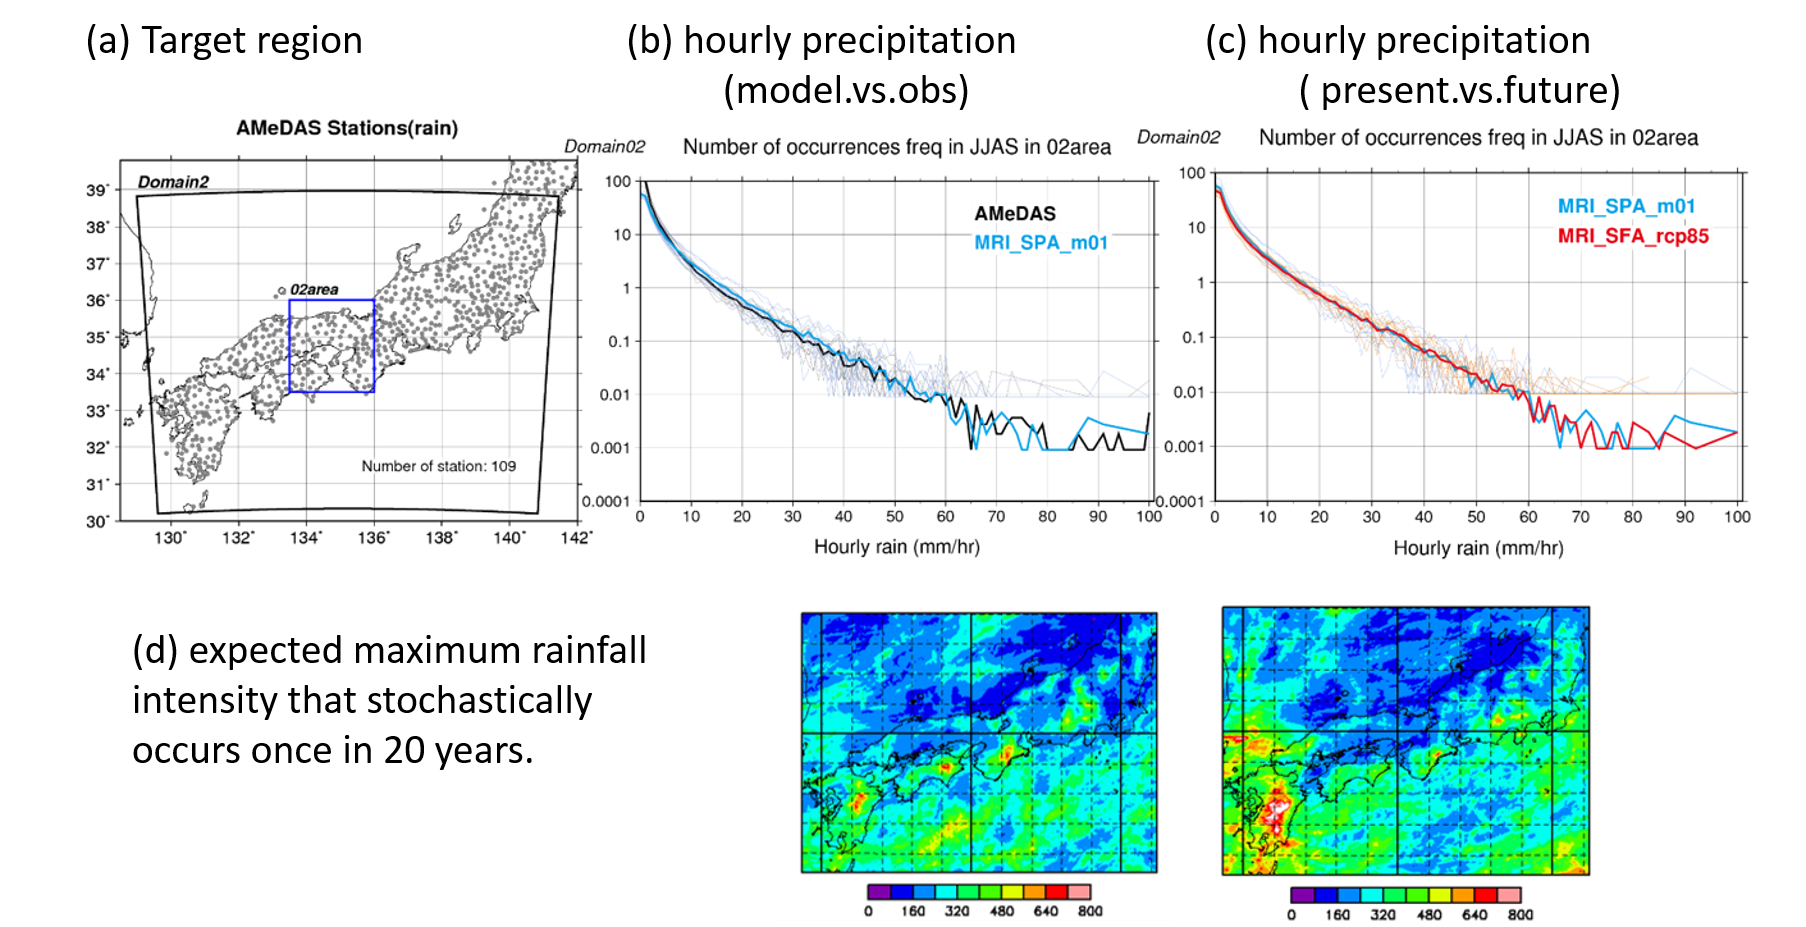
\includegraphics[width=1.0\textwidth,keepaspectratio,natwidth=193,natheight=40]
  {research/tomita/climate-teamFig3.png}
  \caption{The result of the preciptation property in the Japan/Kansai region by the direct downscaling.}
  \locallabel{fig:ctfig3}
\end{figure}


%Text for research Results and achievements. Journal-artcile~\cite{sample-journal}.
%Conference-paper~\cite{sample-conference}.
%Invited-talk~\cite{sample-invited}.
%
%%For cross referencing, use \verb|\locallabel| and \verb|\localref| to avoid conflicting names defined by other groups. For example, a figure can be referenced as Figure~\localref{fig:sample-label1}.

%\begin{figure}
%\centering
%  \includegraphics[width=0.5\textwidth,keepaspectratio,natwidth=193,natheight=40]
%  {sample_division/sample_group/test1.png}
%  \caption{Caption for a sample figure}
%  \locallabel{fig:sample-label1}
%\end{figure}

\section{Schedule and Future Plan}

In the next year, we will continue to further develop, update and maintain the numerical library for the K computer (SCALE library). We also try to enhance the performance of each existing scheme. Especially, validation of cumulus parameterization is necessary. At the same time, we will work on the following three projects in the collaboration with other team in AICS and the scientist in other institute.
\begin{enumerate}
\item On the Hyogo/Kobe COE establish project, we will continue the long-term climate simulation by using SCALE-RM to examine the heavy rainfall over Kobe city area. Several MRI-AGCM results for the future climate is used for increase of scenarios. We will obtain the geographical distribution of the frequency of heavy rainfall and evaluate it more precisely. For this purpose, the pseudo global warming method will be also employed. 
\item We will also contribute to the CREST, Strategic Basic Research Programs “Innovating "Big Data Assimilation" technology for revolutionizing very-short-range severe weather prediction” to develop the main climatological model in SCALE library. In collaboration with the Data Assimilation team in AICS, we developed a prototype of SCALE-LETKF (Local Ensemble Transform Kalman Filter). For this short range forecast, we will pursue both of the computational and physical performance.
\item We join the POST K Science priority project under the collaboration with JAMSTEC. NICAM-LETKF is one of the target applications. Our team will continue to develop and update that application.
\end{enumerate}

%Text for schedule and future plan.
%%
%%


%%% DO NOT EDIT BELOW

\section{Publications}

%\printbibliography[keyword=journal, heading=subbibliography, title={Journal Articles}, prefixnumbers={1-}, resetnumbers=true]
%\printbibliography[keyword=proceedings, heading=subbibliography, title={Conference Papers}, prefixnumbers={2-}, resetnumbers=true]
%\printbibliography[keyword=invited, heading=subbibliography, title={Invited Talks}, prefixnumbers={3-}, resetnumbers=true]
%\printbibliography[keyword=poster, heading=subbibliography, title={Posters and Presentations}, prefixnumbers={4-}, resetnumbers=true]
%\printbibliography[keyword=deliverable, heading=subbibliography, title={Patents and Deliverables}, prefixnumbers={5-}, resetnumbers=true]

\printbibliography[keyword=journal, heading=subbibliography, title={Journal Articles}, resetnumbers=true]
\printbibliography[keyword=proceedings, heading=subbibliography, title={Conference Papers}]
\printbibliography[keyword=invited, heading=subbibliography, title={Invited Talks}]
\printbibliography[keyword=poster, heading=subbibliography, title={Posters and Presentations}]
\printbibliography[keyword=deliverable, heading=subbibliography, title={Patents and Deliverables}]

\end{refsection}
